\documentclass[AEJ, finalmode]{AEA}

%\usepackage[cmbold]{mathtime}
\usepackage[abbr]{harvard}
\usepackage{amsmath}
\usepackage{graphicx}
\usepackage{makecell}


\newcommand{\rowgroup}[1]{\hspace{-1em}#1}
\draftSpacing{1.5}
\begin{document}


\title{Historical Lynchings and the Contemporary Voting Behavior of Blacks}
\shortTitle{Lynchings and Voting of Blacks}
\author{Jhacova Williams\thanks{RAND Corporation, 1200 S Hayes St. Arlington, VA 22202 (email: jwillia@rand.org). Many thanks to Naci Mocan, Chris Foote, Trevon Logan, Lisa Cook, Louis-Philippe Beland, Breyon Williams, Falk Brauning, Osborne Jackson, Geoffrey Tootell, Robert Margo, Ebonya Washington, Ross Hallren, Tamara Gurevich, Gary Hoover, Gregory Price, Jori Kandra and seminar participants of the Southern Economic Association Conference in Washington D.C., the Federal Reserve Bank of Boston, the United States International Trade Commission, and the CSMGEP Dissertation Session for useful comments and discussions.}}
\date{\today} 
\pubMonth{Month}
\pubYear{Year}
\pubVolume{Vol}
\pubIssue{Issue}
\JEL{N90, J15, Z10}


\begin{abstract}
This paper analyzes the extent to which the political participation of blacks can be traced to historical lynchings that took place from 1882 to 1930. Using county-level voter registration data, I show that blacks who reside in southern counties that experienced a relatively higher number of historical lynchings have lower voter registration rates today. This relationship holds after accounting for a variety of historical and contemporary characteristics of counties. There exists evidence of the persistence of cultural voting norms among blacks yet this relationship does not exist for whites.  
\end{abstract}

\maketitle

``A lynching is much more than just a murder. A murder may occur in private. A lynching is a public spectacle; it demands an audience...A lynching is a majority's way of telling a minority population that the law cannot protect it." - Aatish Taseer, \textit{Anatomy of a Lynching} (2017) 

\vspace{5mm}
Political participation is one of the most fundamental ways in which citizens participate in the democratic process. In theory, it allows each citizen an equal voice in American politics and thereby an equal voice in American public policy. Yet more than fifty years following the enactment of the Voting Rights Act of 1965, the political participation of blacks remains lower than that of whites in many elections in the United States.\footnote{The Voting Rights Act of 1965 prohibited voter-discrimination schemes that prevented blacks from participating politically \cite{christopher1965constitutionality}.} Considering that blacks are underrepresented in political participation, thereby causing their interests to be underrepresented in American public policy, examining explanations for low political participation among blacks can be used to inform policy.\footnote{\citeasnoun{miller2015elections} states that politicians who depart from citizens’ interests are more likely to be replaced. Since the black population is not large enough to control legislative bodies in any state, their “policy preferences become only public only if supported by a coalition of black and white representatives \cite{bullock1981policy}.”}

In this paper, I propose an explanation that explores a setting that experienced violent racist acts in the past - the American South. Specifically, I ask whether historical racial animus continues to influence the voting behavior of blacks. Using historical lynchings, a general indicator of the extent to which a county was able to inflict violence on blacks \cite{jones2017political} to proxy racial animus, I test whether there exists a link between historical lynchings and the contemporary political participation of blacks.\footnote{Recent findings have argued that violence in political settings can create mistrust in the government which may cause individuals to avoid the political process \cite{blanco2013impact,jones2017political}. When viewed as a general indicator of violence, \citeasnoun{jones2017political} propose that lynchings would have a ``\textit{persistent and lasting effect on voter turnout}".} Considering that historical lynchings were mechanisms for social control that discouraged a variety of activities among blacks including voting \cite{dickerson2003reconstruction,cook_logan_parman} recent findings of habit-formation and norm-based voting \cite{gerber2003voting,dellavigna2016voting,fujiwara2016habit} and the strong correlation between parent and child's voting propensity \cite{akee2018}, it is plausible that past events continue to influence the political participation of blacks today.\footnote{ \citeasnoun{dellavigna2016voting} find that individuals are motivated to vote due to the social image received from family and friends. \citeasnoun{gerber2003voting} and \citeasnoun{fujiwara2016habit} show that voting is a habitual act based on previous voting conditions and experiences. \citeasnoun{akee2018} find an intergenerational transmission of voting behavior in that there exists a strong correlation between parents' prior voting propensity and their children's voting propensity in the future.} 

To investigate whether historical racial animus continues to influence the political participation of blacks, I combine county-level lynching data with contemporary voter registration data. After accounting for a variety of historical characteristics of counties, the results show that blacks who reside in counties that were exposed to a relatively higher number of lynchings from 1882 to 1930 have lower voter registration rates today.

A number of falsification exercises show the robustness of this basic correlation in that lynchings are not related to the voting behavior of whites. Motivated by the possibility that slavery left behind anti-black institutions that reduce the political participation of blacks today \cite{acharya2015culture}, I include an additional specification that accounts for an area's historical prevalence of slavery. Additionally, this negative relationship may be due to  contemporary measures such as education, earnings, high incarceration rates of blacks, and the paucity of polling places in counties. The results remain virtually unchanged after the inclusion of these potential confounders.


While the goal of this paper is to estimate the long-run association of the political participation of blacks and a historical proxy for racial animus, it is impossible to distinguish whether this is due to the persistence of cultural voting norms that have been transmitted to subsequent generations or the persistence of discriminatory acts that prevent blacks from voting today. However, the analysis to follow will test several likely mechanisms and finds evidence of the transmission of cultural voting norms among blacks. 


The first mechanism I examine is whether the relationship between historical lynchings and the voting behavior of blacks is due to geographic sorting. For example, during the Great Migration, blacks with higher voting propensities may have migrated away from violent southern areas while blacks who were less likely to participate in voting remained. Using data from the 1940 100\% IPUMS-USA \cite{ipumsacs}, I examine whether black migrants out of southern counties with higher lynching rates differ from individuals who did not migrate from these counties. I find no evidence of geographic sorting as a function of lynching rates which suggests that the relationship between lynchings and voting behavior of blacks is not explained by sorting.


The next mechanism I examine is whether counties with a relatively higher number of historical lynchings have contemporary barriers that suppress the voting of blacks. For instance, if counties that experienced more historical lynchings also have fewer polling places in areas where blacks live today, then the results may be an artifact of this phenomenon. To understand whether the paucity of polling places in black areas explains the relationship between lynchings and the voting behavior of blacks, I use data on polling locations.\footnote{Polling location data are obtained from the Secretary of State Offices in 2017 and reflect polling place locations in the 2016 Presidential Election. Data come from \citeasnoun{sosalpoll}, \citeasnoun{sosflpoll}, \citeasnoun{sosgapoll}, \citeasnoun{soslapoll}, \citeasnoun{sosncpoll}, and \citeasnoun{sosscpoll}.} I find no evidence that counties with a relatively higher number of historical lynchings have fewer polling places in areas where blacks reside.


The final mechanism I examine is whether lynchings are related to cultural voting norms among blacks. If lynchings discouraged the political participation of blacks in the past, thereby causing blacks to become disinterested in participating, this behavior may have been passed down to future generations. Using data from \citeasnoun{sfp}, I examine whether lynchings are related to voting norms among blacks. I find that blacks who reside in areas with a relatively higher number of lynchings are less likely to indicate that their parents felt it was important for them to be patriotic yet this relationship does not exist for whites.


After identifying a potential mechanism for the relationship between historical lynchings and the contemporary political participation of blacks, I examine whether the relationship between lynchings and black political participation can be mitigated. For example, \citeasnoun{tate1991black} found that blacks with higher income, more education, and stronger social ties to the black community were more likely to participate in voting. To investigate this, I interact lynching rates with county-level measures of earnings, education, and the black church member rate.\footnote{The black church member rate is the number of members that attend churches with predominate black congregations per black 10,000 population in 2010.} The results show that education and earnings do not change the relationship between lynchings and voting. However, the relationship between lynchings and political participation is mitigated by higher rates of black church members. 


There are two main contributions of this paper. First, it adds to recent findings in economics by helping us understand how an initial shock that alters behavior can have a persistent impact \cite{nunn2011slave,acemoglu2012colonial,voigtlander2012persecution,acharya2016political}. Second, the paper increases our understanding of the determinants of voting by measuring the extent to which violent acts can deter the target group from voting in the future.

This paper is organized as follows. Section I provides the historical background and conceptual framework. The data description is given in Section II. The empirical framework, presented in Section III, is used to motivate the empirical analysis to follow. Section IV presents the results. Section V examines potential mechanisms and Section VI concludes.

\section{Historical Background and Conceptual Framework}
\subsection{Historical Background}

The Reconstruction Act of 1867 forever changed the voting population in the South with Congress requiring Southern conventions to met and adopt new constitutions that included manhood suffrage \cite{dubois1935black,foner1988reconstruction}. With this enactment, more than one million blacks and more than 300,000 illiterate, poor whites were given the right vote \cite{dubois1935black}. Manhood suffrage was supported by Union army commanders who sought to protect any devices that would keep blacks from the polls \cite{dubois1935black}. Also, officials from the Freedmen's Bureau ``\textit{advised Negros about registration and voting and disabused their minds of fears of taxation or military service or reenslavement}" \cite{dubois1935black}. These measures of protection resulted in voter turnout among black men that ranged between 70\% and 90\% \cite{kent2003making} and restructured the South. Blacks voted for white Republican politicians who filled seats once held by Democrats as well as black men held political office for the first time. For example, blacks were 61\% of the state delegates in South Carolina, 50\% of the state delegates in Louisiana, and 40\% of the state delegates in Florida \cite{dubois1935black}. 

While these elections were the most democratic ever seen in the South \cite{dubois1935black}, some individuals were not pleased by this restructuring. Violent intimidation from the Ku Klux Klan (KKK) in the form of beatings, burnings, and lynchings was used to discourage blacks from voting \cite{defina2011legacy}. During the Presidential campaign season of 1868, KKK members rode around on horses wearing white hoods and robes threatening blacks that if they did not vote for the Democratic ticket, they would be lynched \cite{dickerson2003reconstruction}.\footnote{In 1871, Congress appointed a committee to investigate allegations of voter intimidation \cite{tolnay1995festival}. ``Witnesses repeatedly testified that during the late 1860s a surge of terrorism was directed against politically active blacks." Shaffer Bowens, a Ku Klux Klan member, testified during these hearings that the aims and methods of the Klan was ``to advance the conservative party and put down the radical party….By killing, and whipping, and crowding out men from the ballot boxes."} In 1868, the KKK killed more than 2,000 blacks in Louisiana, two South Carolina legislators, and the President of the Union League, causing black voter turnout to be reduced by 20 percent between the 1867 and the 1868 election \cite{dickerson2003reconstruction,jones2017political}.\footnote{The Union League was an organization that helped blacks register to vote and was headed by northern Republicans. Additionally, these acts of terror reduced voter turnout in additionally southern states. Jones et al. (2017) find that exposure to lynchings reduced black voter turnout by 2.5 percentage points in the post-Reconstruction south.} These KKK terrorists' acts helped the south regain Democratic control in the statehouse in 1870 \cite{dickerson2003reconstruction}. 

While lynchings continued after the 1868 election, lynchings were not restricted to political intimidation. In fact, there exist three theories to explain lynching behavior. The first theory hypothesizes that blacks were lynched because they were seen as an economic threat \cite{beck1992season,cook_logan_parman}. By lynching blacks, whites vented economic frustration due to inflation or decreases in cotton prices \cite{defina2011legacy} and instilled fear in blacks who could compete for jobs \cite{cook_logan_parman}. The second theory hypothesizes that blacks were lynched because they were viewed as a social threat \cite{price2008does,cook_logan_parman}. \citeasnoun{cook_logan_parman} state that whites feared losing their social status to blacks and used lynching as a way of maintaining social order. The third theory, \citeasnoun{blalock1967toward} power threat hypothesis, proposed that violence arouse when the dominant group perceived the subordinate group contested their political authority \cite{price2008does}. Figure~\ref{histreg} supports \citeasnoun{blalock1967toward} power threat hypothesis in that areas with higher percentages of black registered voters in 1867 also had higher lynching rates during the lynching period.\footnote{This figure is created using a binned scatter plot which controls for the percentage of black residents (to total residents) in 1860. OLS results can be found in the online Appendix Table B1.}  

According to \citeasnoun{allen2000without}, blacks were aware of lynchings that took place by the depiction of lynchings in newspapers and on postcards. Figure~\ref{totalmap} presents a county-level mapping of the total number of lynchings between 1882 and 1930 and shows that some counties experienced as many as 25 lynchings during this time period with variation across counties and states.\footnote{A map of lynchings is presented for county state pairs that have voting data separated by race namely Alabama, Florida, Georgia, Louisiana, North Carolina, and South Carolina.} Yet, examining the number of lynchings may not accurately depict the ``threat of violence" since it does not account for an area's size. As such, Figure~\ref{totalnormmap} presents the total number of lynchings normalized by black population in 1900. The map shows that lynching rates were as high as 159.82 per 10,000 black residents in 1900. 

This southern racial climate, along with low voter registration among blacks, continued well into the mid-1900s. For example, in 1940 black registration in eleven southern states was estimated to be 151,000, which was approximately 3\% of the 5 million southern blacks who were of voting age \cite{garrow1978protest}. While some southern states saw increases in black registration in the late 1950s and early 1960s, three states with the majority of voting discrimination lawsuits saw no significant increases in black registration - Alabama, Louisiana, and Mississippi \cite{garrow1978protest}. Efforts to prevent voter discrimination lacked the coercive capabilities to guarantee full civil rights, which caused Congress to pass ``the most significant civil rights landmark of our time" \cite{byrne2005unfinished} - the Voting Rights Act (VRA) of 1965. 

The VRA prohibited barriers that prevented blacks from registering to vote and resulted in southern states exhibiting increases in black registration after its enactment \cite{cascio2014valuing}. Figure~\ref{proact} shows this fact. The overall voter registration rate among blacks increased in the post-enactment period compared to the pre-enactment period yet despite this increase, lynching rates are negatively associated with black voter registration rates in both periods.\footnote{In 1968, the United States Commission on Civil Rights \cite{proact} published county-level voter registration data by race before and after the enactment of the VRA. Pre-registration data are from 1964 in Alabama, Florida, Louisiana, North Carolina, and South Carolina and from 1962 in Georgia. Post-registration data are from 1967 in Alabama, Georgia, Louisiana, North Carolina, and South Carolina and from 1966 in Florida. The negative relationship remains when the group of outliers are removed from the sample.} This suggests that while the VRA may have eliminated some barriers that prevented blacks from participating politically, the VRA did not eliminate the relationship between racist acts and voter registration among blacks. 

Motivated by the negative relationship between lynchings and black voter registration pre- and post-VRA enactment, the analysis to follow examines whether lynchings continue to influence the contemporary voting behavior of blacks.

\subsection{Conceptual Framework}

The foundational model of voting, developed by \citeasnoun{downs1957economic}, posits that individuals vote when the benefit of voting exceeds the cost.\footnote{Benefit is the probability that an individual's vote will make a difference in the outcome of an election times the utility received from the individual's favorite candidate winning the election, and the payoff an individual receives from exercising his social duty.} Recent models have expanded \citeasnoun{downs1957economic} framework of voting costs to include logistical cost and information cost \cite{matsusaka1995explaining,ashworth2007targeted,charles2013employment}. The logistical cost of voting is the cost associated with the act of voting (e.g. traveling to the poll, waiting in line, etc.) and the information cost of voting is the cost associated with having limited information regarding a candidate or an election \cite{charles2013employment}. 

Within this framework, the historical lynching environment raised the cost of voting for blacks since gathering information on elections as well as traveling to election polls could lead to death for many blacks. Considering that cultural beliefs are viewed as decision-making heuristics or ``rules-of-thumb" which are optimal when information acquisition is either costly or imperfect \cite{nunn2011slave,alesina2013origins}, general beliefs about the ``right" action caused blacks to refrain from voting - thus allowing blacks to save on the cost associated with voting.\footnote{\citeasnoun{jones2017political} state that exposure to violence in a political setting may generate fear and discourage voter turnout.} Within this environment, cultural beliefs about voting were beneficial to blacks, thereby lowering their voting behavior patterns, which may have been passed to subsequent generations. 

A natural question is why would one expect lower voter participation among blacks to be associated with events the occurred nearly 100 years ago. One explanation can be found in the cultural economics literature, which demonstrates that historic events have long-run impacts by permanently affecting culture or norms of behavior.\footnote{For a more detailed discussion, see \citeasnoun{nunnimportance}}. For example, \citeasnoun{nunn2011slave} showed that a culture of mistrust persisted in individuals whose ancestors were heavily targeted during the slave trade in Africa which continues to affect economic development in Africa over 400 years later. \citeasnoun{lowes2018legacy} find that greater historical exposure to campaigns that promoted drugs with negative side effects were associated with lower willingness to receive free tests for anemia or HIV. \citeasnoun{alsan2018tuskegee} find that disclosure to disclosure of the Tuskegee study of 1972 are associated with increases of medical mistrust for older black men. \citeasnoun{mocan2016economic} analyzed whether a culture of racist and xenophobic feelings persisted in Germany following World War II, and found that people who live in states that provided above-median support for the Nazi Party in the 1928 elections have stronger anti-Semitic feelings today. Similarly, \citeasnoun{voigtlander2012persecution} reported a strong positive relationship between violent attacks on Jews during the Black Death in 1348 and support for the Nazi Party in 1928, demonstrating a culture of anti-Semitic views that have persisted more than 500 years. Taken together, research in cultural economics has shown that cultural beliefs are sticky and are transmitted across generations \cite{alesina2013origins}. It is plausible that past lynching events may have caused blacks to avoid the voting process altogether, creating a culture of voter apathy, and these voting norms may have persisted by being transmitted to subsequent generations.\footnote{Due to the lack of voting data by race during the historical time period, this explanation cannot be tested.}

Additional evidence of the persistence of voting behavior can be found in the voting literature. \citeasnoun{akee2018} found that there exists an intergenerational transmission of voting behavior in that there exists a strong correlation between parents' prior voting and their children voting in the future. Additionally, research has shown that voting is habit forming in that voting in one election increases an individual's propensity to vote in future elections. \citeasnoun{gerber2003voting} used a randomized field experiment that randomly assigned individuals to treatment and control groups to isolate the causal role in voting. Individuals in the treatment group were encouraged to vote via mail or via face to face campaigning whereas individuals in the control group were not encouraged to vote. These authors found that this randomized change produced an increase in voting in the upcoming election and increased the likelihood of voting in the future. \citeasnoun{fujiwara2016habit} also showed that voting is habit-forming by empirically disentangling habit formation in voting from other channels of voter persistence. These authors model rainfall, an unexpected and transitory shock, into the cost of voting and find that rainfall on election day decreases voter turnout in the current and future elections. 

While it is plausible that the persistence of voting behavior among blacks exists, it is impossible to distinguish whether lynchings are negatively related to the current political participation among blacks because of the persistence of cultural voting norms or the persistence of discriminatory practices. For instance, areas that were exposed to a higher number of lynchings may have and continue to discriminate against blacks. These practices, in addition to norm based voting, may influence the current voting behavior of blacks. While the analysis below will attempt to examine some of the possible explanations, it is beyond the scope of this paper to fully separate these two mechanisms through which this long-run association exists. Instead, this paper attempts to empirically estimate the long-run association between a proxy for racial animus and the voting behavior of blacks and finds evidence of the persistence of cultural voting norms. 

\section{Data Sources and Description}
The lynching data are obtained from the Historical American Lynching Data Collection Project (Project HAL) and include all lynching victims' records in Southern counties from 1882 to 1930.\footnote{Poject HAL data come from \citeasnoun{hal}. Southern counties include counties in Alabama, Arkansas, Florida, Georgia, Kentucky, Louisiana, Mississippi, North Carolina, South Carolina, and Tennessee.} The Project HAL data include lynchings which meet the NAACP definition.\footnote{To be included in the lynching inventory, an incident must meet the following criteria: a) There must be evidence that someone was killed b) The killing must have occurred illegally c) Three or more persons must have taken part in the killing; and d) The killers must have claimed to be serving justice or tradition.} For each lynching record, the information includes the victim's name, race, gender, and alleged offense.\footnote{Although many of the alleged offenses listed in Project Hal are murder or rape, an 1883 Supreme Court ruling may have influenced what was listed as an alleged offense. This ruling declared it unconstitutional for the federal government to penalize murder or assault and allowed local governments to punish such crimes. The 1883 ruling overturned the 1871 Enforcement Act which granted ``the power of the president to use military force to suppress domestic violence that deprived citizens of their rights, privileges, or immunities, or protection named in the Constitution"  \cite{williams1993south}.} The dataset also includes the county, state, month, day, and year that the lynching occurred.\footnote{Counties that are not listed in Project HAL are assumed to have zero historical lynchings. The results remain when these counties are excluded.} To construct the lynching measure, the data are restricted to black victims and excludes lynchings carried out by black mobs. The lynching measure represents the number of lynchings of black victims that occurred in a county from 1882 to 1930.

I link the aggregated lynching data with population data from the 1900 Census \cite{ipumsnhgis}.\footnote{Considering that the lynching data spans from 1882 to 1930, the year 1900 is nearly the midpoint of the period and is used to normalize the number of lynchings. The results are robust to using the black population in 1910, 1920, or 1930. See online Appendix Table B2.} The 1900 Census population data are obtained from the National Historical Geographic Information System (NHGIS) and contain county-level measures for the black, white, and total population. The lynching and population data are used to construct the main explanatory variable, black lynching rate, which is the number of black lynchings per 10,000 black population in 1900. A lynching rate is constructed as the main explanatory variable as opposed to the number of lynchings since it more accurately captures the intensity of lynchings or ``threat of violence" by accounting for the number of blacks in an area.\footnote{Additionally, previous research used lynching rates rather than the number of lynchings as a measure of violence \cite{cook2014violence,acharya2016political}. }

The voter registration data are obtained from the Secretary of State Offices in Alabama, Florida, Georgia, Louisiana, North Carolina, and South Carolina.\footnote{Registration data come from \citeasnoun{sosal}, \citeasnoun{sosfl}, \citeasnoun{sosga}, \citeasnoun{sosla}, \citeasnoun{sosnc}, and \citeasnoun{sossc}.The data for Alabama, Georgia, Louisiana, and South Carolina are obtained for the years 2000, 2004, 2008, and 2012 due to data availability beginning in many of these states in 2000. Voter registration data in North Carolina are obtained in 2004, 2008, and 2012 since North Carolina does not report race until 2002. The voter registration data in Florida are obtained from its Secretary of State Office in 2016. The method used for extracting voter registration for the years 2000, 2004, 2008, and 2012 is explained in the Data Appendix. Additionally, Georgia, Louisiana, North Carolina, and South Carolina report voter turnout separated by race. The analysis to follow focuses on voter registration since it is available during the historical lynching period, the interim period, and the contemporary period. The results hold when voter turnout is used as an outcome variable.} Ideally, the sample would include all counties in the former Confederate States. However, these are the only states in the former Confederacy, and in the lynching data, in which individuals are asked to identify their race when they register to vote. See Appendix for more information regarding voter registration data from the Secretary of State Offices. 

The voter registration data are merged with population data from the Surveillance, Epidemiology, and End Results Program (SEER) of the National Cancer Institute for the years 2000, 2004, 2008, and 2012.\footnote{Population data come from \citeasnoun{seerpop}. SEER data are used, as opposed to Census data, because population data from SEER can be extracted for Presidential years. SEER data can be broken into postcensal (data after decennial census but before next census) and intercensal (years between two completed decennial censuses) population data. Postcensal population data is estimated by updating resident population in the decennial census using the components of population change approach (births/deaths to U.S. resident women, net international migration, net movement of U.S. Armed forces and civilians, etc.). Intercensal population data is estimated by adjusting the final postcensal estimates for the decade to account for differences between the April 1, base population (from the census at the end of the decade) and the postcensal estimates for April 1 of that census year. See https://www.cdc.gov/nchs/data/series/sr\_02/sr02\_135.pdf or https://www.cdc.gov/nchs/nvss/bridged\_race/Documentation-Bridged-PostcenV2018.pdf for more details.} The SEER data contain county-level population counts by age and race. To focus on individuals who are of voting age, the data are restricted to population counts for individuals who are 18 or older. The registration and SEER data are used to construct the outcome measure, voter registration rate, as the county-level percentage of black registered voters per black voting age population. Similarly, voter registration rate among whites is measured as the percentage of white registered voters per white voting age population.\footnote{Voter registration rate is more than 100\% in some counties. The results to follow use voter registration as is. The results when voter registration rates are top-coded to 100 and when counties with voter registration rates that exceed 100 are removed from the sample can be found in the online Appendix Table B3.}

The primary source for historical measures in this study is the NHGIS \cite{ipumsnhgis} which provides Census data from 1790 to the present. Proxies for historical institutional quality include the newspaper rate in 1840 and the year in which a county was formed \cite{grosjean2014history}.\footnote{Newspapers have been shown to be a good proxy for institutional quality. \citeasnoun{gentzkow2006rise} find that when corruption declined in the US, between 1870 to 1920, the press expanded its circulation. \citeasnoun{besley2002political} find that newspaper circulation is related to the dispersion of food aid and calamity relief in India. \citeasnoun{besley2006handcuffs} show that higher rates of state ownership of newspapers is associated with higher levels of corruption.} To capture historical economic indicators, I include the average farm value \cite{ipumsnhgis}, the proportion of small farms and land inequality in 1860 \cite{acharya2016political}.\footnote{Data on land inequality come from \citeasnoun{acharya2016political} as originally obtained from \citeasnoun{nunn2008slavery}.} Additionally, the proportion of free blacks in 1860 is included to proxy norms about race \cite{acharya2016political}. The number of black illiterate men per black voting age population is obtained from the 1910 Census \cite{ipumsnhgis}. See Data Appendix for detailed information regarding historical controls. 

Table~\ref{statistics} presents the Descriptive Statistics. Although Table~\ref{statistics} shows that the voter registration rate of blacks is close to that of whites with rates of 73.85\% and 76.29\% respectively, this phenomenon is a result of high voter registration rates and voter turnout among blacks in the 2008 and 2012 Presidential Elections.\footnote{The 2008 and 2012 Presidential Elections included the first African American Presidential Nominee, Barack Obama.} While voter registration rates among blacks (whites) exceed 100\% in some counties, the result remains when these counties are excluded from the sample or when they are top-coded at 100\%.\footnote{Voter registration rates of blacks exceeds 100\% in 8 of the 267 counties in the sample.} 

\section{Empirical Framework}

To estimate the relationship between historical lynchings and the contemporary voting behavior of blacks, the baseline equation estimates the following equation: 
\begin{equation}
\begin{aligned}
voter\;registration\;rate_{cs} = & \beta_{0} + \beta_{1}lynching\;rate_{cs} \\  & + \beta_{2}X^H_{cs} + \delta_{s} + \epsilon_{cs}
\label{olsbaseline}
\end{aligned}
\end{equation}
where $c$ indexes counties and $s$ indexes states; $voter\;registration\;rate_{cs}$ is the averaged percentage of black registered voters per black voting-age population in the 2000, 2004, 2008, and 2012 Presidential Elections; $lynching\;rate_{cs}$ is the number of lynchings of blacks from 1882 to 1930 per 10,000 black population in 1900.\footnote{This measure excludes lynchings performed by black mobs against blacks.} $X^H_{cs}$ represents the vector of observed historical county characteristics that vary across counties. This vector includes factors that may have been determinants of lynchings, namely economic, institutional, social, and political factors.\footnote{See Section II for theories of lynchings.} To account for economic indicators, similar to \citeasnoun{acharya2016political}, I include the average farm value in 1860, the proportion of small farms in 1860, and land inequality in 1860. Similarly, to account for social factors, I include the proportion of free blacks in 1860 to proxy norms of race \cite{acharya2016political}. My specification differs from \cite{acharya2016political} in that I include proxies for institutional quality such as the average number of newspapers per total population in 1840 and the year in which a county was formed \cite{grosjean2014history}. Barriers to voting during the historical period included polling taxes and literacy tests. However, these barriers were instituted at the state-level in Southern counties. To proxy political barriers, I include the number of black illiterate men per 10,000 voting age population in 1910. This variable is included since it is reasonable to believe that barriers to voting were implemented differently in areas with smaller (or larger) shares of illiterate black voters. $\delta_{s}$ is the set of state fixed effects and $\epsilon_{cs}$ is the error term. The main coefficient of interest, $\beta_{1}$, estimates the impact of one additional lynching per 10,000 black population in 1900 on the percentage of black registered voters per black voting-age population. 


\section{Results}

Figure~\ref{baseline} shows the relationship of Equation (1). The dependent variable, voter registration rate of blacks, is defined as the percentage of black registered voters per black voting-age population. Figure~\ref{baseline} shows that lynching rates are negatively associated with black voter registration rates.\footnote{The negative relationship remains when the group of outliers are removed from the sample. Additionally, examining the sensitivity of the results to various specifications shows that the negative relationship remains when the lynching rate uses a log or arcsin transformation and when the lynching rates in the 95th percentile are dropped from the sample. However, dropping the 95th percentile lynching rates loses significance.} Specifically, moving from the 25th percentile of lynching rates to the 75th percentile of lynchings rates results in a 2.2 percentage point difference (equivalent to a 2.7\% change) in voter registration rates among blacks.\footnote{The difference in voter registration rates between whites and blacks differs by 5.7, 9.1, 3.8. and 0.6 percentage points in the 2000, 2004, 2008, and 2012 elections respectively (Census Bureau Voting and Registration in the Election).} This suggests that blacks who reside in counties that were exposed to a relatively higher number of historical lynchings are less likely to register to vote today. 

\subsection{Falsification Exercises}

Next, I perform a number of falsification exercises. First, I consider whether there exists a relationship between lynching rates of whites and the contemporary voting behavior of blacks. Considering that blacks were disproportionately lynched compared to whites following the American Civil War (Price et al. 2008) and lynchings are proxies for historical racial animus towards blacks, there should not exist a significant relationship between lynching rates of whites and the voting behavior of blacks. Table~\ref{falsifications} shows the results. Column (1), which is used for comparison purposes, presents the baseline estimate of the relationship between black lynching rates and registration rates among blacks. Column (2) presents the estimates using white lynching rates. Column (2) shows that the estimates are close to zero and statistically insignificant indicating that lynching rates of whites cannot be linked to the contemporary voting behavior of blacks. 

Second, I consider whether there exists evidence of a relationship between lynching rates and the contemporary voting behavior of whites using black and white lynching rates in Columns (3) and (4) of Table~\ref{falsifications} respectively. Similar to the previous falsification exercise, black lynching rates and whites lynching rates are not related to the contemporary voting behavior of whites. In fact, the estimates are close to zero and statistically insignificant. The results from Table~\ref{falsifications} show that lynching rates of blacks are only associated with the contemporary voting behavior of blacks - the targeted group of 90\% of lynchings. 

\subsection{Robustness Checks}

Motivated by the possibility that this relationship may be explained by several characteristics of counties, I examine a number of potential confounders. First, I examine whether this relationship is robust to the inclusion of slavery.\footnote{\citeasnoun{acharya2015culture} found that slavery left behind formal and cultural institutions (i.e. black codes, racial violence, Jim Crow, etc.), which made it difficult for blacks to vote, and continues to affect voter turnout of blacks today.}

As seen in \citeasnoun{acharya2015culture}, I include the slave rate in 1860 \cite{ipumsnhgis} to serve as a proxy for institutional structures that may make it difficult for blacks to vote today. Column (1) of Table~\ref{slaves} shows the baseline estimates and Column (2) accounts for the number of slaves per 10,000 total population in 1860. Contrary to \citeasnoun{acharya2015culture}, the number of slaves is positively associated with voter registration rates of blacks, and this association is significant at the 1\% level. To examine the discrepancy between the results in Column (2) and the results in \citeasnoun{acharya2015culture}, I examine whether current shares of black populations can explain this difference. For example, if current shares of blacks who are of voting age are positively associated with the share of slaves in 1860, then this positive association may be the result of blacks being more likely to register in areas in which there are more ``like-minded" individuals. While a simple method to examine this would be to control for the contemporary share of voting age blacks (i.e. the number of voting age blacks per total voting age population), the outcome variable, registration rates of blacks, is defined as the percentage of black registered voters per black voting age population. Hence, controlling for the contemporary share of voting age blacks would lead to simultaneous bias. 

To examine whether this relationship explains the positive association between slavery and the contemporary voter registration of blacks, I employ two methods. First, I examine the relationship between the share of slaves and the share of voting-age blacks. Figure~\ref{scatblackslaves} depicts the scatter plot of these two variables and shows a positive association between the share of slaves and the current share of voting age blacks. Figure~\ref{binblackslaves} shows the binned scatter plot which again depicts a positive association between the share of slaves and the share of voting-age blacks. The second method changes the main specification so that the outcome variable is the number of black registered voters rather than the black registration rate (i.e. it is not normalized by the black voting age population) and controls for the current rate of voting age blacks. The results can be seen in Table~\ref{regblack}. The results show two facts. First, similar to \citeasnoun{acharya2015culture}, slavery is negatively associated with the number of registered blacks, and the current rate of voting age blacks is positively associated with the number of blacks registered to vote. Second, there does not exist a statically significant relationship between slavery and current levels of registered blacks voters yet there exists a statistically significant relationship between the voting age blacks and the level of registered black voters. Taken together, the methods employed suggest that the positive coefficient seen in Table~\ref{slaves} Column (2) can be explained by blacks being clustered in areas the had a higher prevalence of slavery in the past. 

Next, I examine whether the relationship between lynchings and the political participation is robust to contemporary factors. Table~\ref{lynchmob} Columns (1) - (5) accounts for each potential confounder by adding each confounder to the baseline specification.\footnote{See data appendix for a discussion of data sources for each variable.} 

Since education and earnings have been shown to be associated with political participation, Columns (1) and (2) include education and earnings into the baseline specification respectively.\footnote{Earnings data come from \citeasnoun{qwiearn} and education data come from \citeasnoun{ipumsnhgis}.} The results show that there exists a positive yet statistically insignificant relationship between education and voter registration as well as earnings and voter registration. 
 

Because blacks have higher incarceration rates compared to other racial groups and individuals cannot vote when they are incarcerated, Column (3) incorporates incarceration rate of blacks into the baseline specification.\footnote{Incarceration data come from \citeasnoun{incarceration}. In Georgia, Louisiana, North Carolina, and South Carolina ex-offenders can register to vote after completion of their full sentence. In Alabama, ex-offenders can register to vote after completing their entire sentence except those convicted of murder, rape, incest, sexual crimes against children, and treason. In Florida, ex-offenders can register to vote 5 years after completing their sentence except those convicted of murder, assault, child abuse, drug trafficking, and arson. Ex-offenders convicted of these crimes can register to vote 7 years after completing their full sentence. One limitation with this data is that the incarceration rate is based on the number of individuals in local jails not incarcerated individuals' home addresses.} The results show that the incarceration rate is negatively associated with voter registration rates yet this association is insignificant. 

The number of polling places, which has been shown to positively affect voter participation, can be viewed as a proxy for accessibility to voting. Column (4) includes the polling place rate into the baseline specification.\footnote{Polling place data come from \citeasnoun{sosalpoll}, \citeasnoun{sosflpoll}, \citeasnoun{sosgapoll}, \citeasnoun{soslapoll}, \citeasnoun{sosncpoll}, and \citeasnoun{sosscpoll}.} The results show that the number of polling places is positively and significantly associated with voter registration rates of blacks. This indicates that easier access to voting, in the form of polling places, increases registration rates of blacks. 

The final column of Table~\ref{lynchmob} presents the specification which includes all potential confounders, historical controls and state fixed effects. The results show that for one additional lynching per 10,000 black population in 1900, the voter registration rate of blacks decreases by 0.34 percentage points and this result is significant at the 5\% level. In other words, moving from the 25th percentile of lynching rates to the 75th percentile of lynchings rates results in a 1.5 percentage point difference (equivalent to a 2.03\% change) in voter registration rates among blacks.

In summary, Table~\ref{lynchmob} shows that there exists a link between historical lynchings and the contemporary voting behavior of blacks.\footnote{An additional specification uses lynching data from the Equal Justice Initiative (EJI) which contain county-level lynching from 1877 to 1950. The results remain negative and significant and can be seen in the online Appendix Table B4.} Additionally, while the results are robust to the inclusion of the potential confounders, some or all of these controls are endogenous in that they could be affected by lynchings. As a result, the remainder of the analysis will use the baseline specification as the preferred specification. This specification includes historical controls and state fixed effects.\footnote{Considering that the estimates obtained in Table~\ref{lynchmob} may be biased by unobservables, I examine whether selection on observables can be used to access the potential bias from unobservables \cite{altonji2005selection,oster2017unobservable}. The results show that selection on observables is unlikely and can be seen in online Appendix Table B5.} 


\section{Mechanisms}

Up to this point, I have shown that lynchings are associated with the contemporary voting behavior of blacks. This relationship is consistent with the hypothesis that historical racial animus continues to influence the political participation of blacks. Yet, an explanation for this relationship has not been identified. In this section, I perform a number of exercises to identify potential channels though which this relationship might exist. 

\subsection{Migration Results}

The first potential explanation examines whether these results can be explained by geographic migration. For example, during the Great Migration, which lasted from 1916 to 1970, millions of blacks migrated away from southern states to northern and western states in search of better economic and social conditions. If blacks who were more likely to participate in voting were also more likely to migrate away from violent southern counties, blacks with lower voting propensities remained.

Following \citeasnoun{acharya2016political}, I use the 1940 100\% sample obtained from the IPUMS-USA \cite{ipumsacs}. This sample is unique in that it provides a respondent's current county of residence as well as the county of residence five years prior (Acharya et al. 2016) allowing for individuals who migrated from southern counties to be identified. Once identified, I can test whether migrants' individual attributes differ from individuals who remained in southern counties. For geographic sorting to explain the results, patterns of mobility out of southern counties would need to differ as a function of lynchings.   

To examine whether geographic sorting explains the results, I restrict the data to blacks and estimate:
\begin{equation}
\begin{aligned}
attributes_{i} = & \gamma_{1}outmigration_{i} + \gamma_{2}lynching\;rate_{1935i} \\ & +  \gamma_{3}(outmigration_{i}*lynching\;rate_{1935i}) \\ & + \gamma_{4}X^H_{1935cs} + \delta_{1935s} +  \epsilon_{ics},
\end{aligned}
\label{migrationequ}
\end{equation} 
where $attributes_{i}$ represents a respondent's wage, age, gender, education level, weeks worked, and rent; $outmigration_{i}$ represents whether an individual migrated out of a southern county.\footnote{Southern counties include counties in Alabama, Florida, Georgia, Louisiana, North Carolina, and South Carolina.} This regression also includes historical controls based on a respondent's 1935 county of residence and his or her 1935 state fixed effects. The main coefficient of interest, $\gamma_{3}$, estimates differences between out-migrants' individual attributes and those who did not migrate as a function of the lynching rate. Table~\ref{migrationtable} shows the results from Equation (2). We see that out-migrants have lower wages, are older, are less likely to be female, are more likely to have 9th grade education or more, are more likely to be full-time, and have lower rent compared to individuals who ``stayed" in southern counties with higher lynching rates. However, these estimates are close to zero and are statistically insignificant.\footnote{Females are less likely to be out-migrants compared to stayers in southern counties with higher lynchings rates and this relationship is statistically significant.} 

Considering the data used in Equation (2) cover a small window during the Great Migration, I use data from \citeasnoun{collins2014selection} to examine black male southern migrants and non-migrants during the peak of the Great Migration (1910 to 1930). Using data from \citeasnoun{collins2014selection} support the results seen in Table~\ref{migrationtable} in that black male migrants do not differ significantly from non-migrants on selected attributes and the estimates are close to zero. These results can be found in online Appendix Table B6. Together, these findings suggest that sorting does not explain the relationship between lynching and the voting behavior of blacks. 

\subsection{Polling Locations}

The second explanation examines whether counties that experienced a relatively higher number of lynchings have contemporary barriers that suppress voting. I consider one potential barrier - the paucity of polling places in black areas. That is, I examine whether counties with more historical lynchings have fewer polling places in areas where blacks live. If the number of polling places varies as a function of lynching rates and the proportion of blacks in an area, then my results may be a result of this phenomenon. However, if no relationship exists, then this exercise will strengthen the claim that historical lynchings, a proxy for historical racial animus, have had a long-run association with the voting behavior of blacks.

To examine this relationship, I obtain the GIS boundary census-tract map along with census-tract population data from the 2010 Census \cite{ipumsnhgis}. Polling place data come from the Secretary of State Offices in Alabama, Florida, Georgia, Louisiana, North Carolina, and South Carolina and includes the name of each polling place, each polling place address, and county and state identifiers. Using an address locator from ArcGIS, each polling place address is geocoded into its equivalent latitude and longitude coordinate. As shown in Figure~\ref{map}, pairs of coordinates are overlaid onto the 2010 United States census-tract boundary map \cite{ipumsnhgis}. Figure~\ref{mapzoom} shows an enlarged mapping of geocoded addresses in Louisiana and shows that the number of polling places varies across census-tracts. 

Using this mapping, I tally the number of polling places that lie within the GIS census-tract and merge this dataset with the 2010 population data and the lynching data to be used in Equation (3).\footnote{To merge the geocoded address (point) layer with the NHGIS census-tract boundary layer, I use the intersect tool in ArcGIS. The intersect tool takes two layers as input and returns the features that belong to both layers as output. Census-tract boundaries that do not contain any points from the point layer are assumed to have no polling places. The merged point and boundary layer file is aggregated to the census-tract level which yields the total number of polling places in each census tract.}

To examine whether the number of polling places varies as a function of the proportion of blacks and the lynching rate, I consider:
\begin{equation}
\begin{aligned}
polling_{t} = & \kappa_{0} + \kappa_{1}share\;black_{t} + \kappa_{2}lynching\;rate_{c} + \\ & \kappa_{3}(share\;black_{t}*lynching\;rate_{c}) + \kappa_{4}population\;density_{t} + \epsilon_{t}
\end{aligned}
\label{pollequ}
\end{equation}
where $polling_{t}$ is the number of polling places per 10,000 population which varies across census tracts, $share\;black_{t}$ is the proportion of blacks which varies across census tracts, $lynching\;rate_{c}$ is the number of black lynchings from 1882 to 1930 per black population in 1900 which varies across counties, and $population\;density_{t}$ is the population per 100 land area which varies across census tracts.\footnote{Land area is measured in square miles.} The coefficient of interest, $\kappa_{3}$, measures the relationship between lynchings and the number of polling places as a function of the proportion black. Table~\ref{tract} shows three facts. First, areas with a larger proportion of black residents have fewer polling places, yet the association is insignificant and the coefficient is close to zero. Second, areas that experienced a relatively higher number of lynchings in the past have fewer polling places today. This association is significant at the 1\% level yet the magnitude of the estimate is negligible. Finally, there is no significant difference in the number of polling places as the proportion of blacks and the lynching rate vary. In fact, the magnitude of the main coefficient of interest, $\kappa_{3}$, is close to zero. In summary, Table~\ref{tract} suggests that there does not exist evidence that counties that experienced a relatively higher number of lynchings have fewer polling places in areas where blacks reside.

\subsection{Cultural Voting Norms}

The final explanation examines whether lynchings are related to cultural voting norms of blacks. Considering that research has shown that individuals are motivated to vote due to the social image received from family and friends \cite{dellavigna2016voting}, it is plausible that lynchings created persistent cultural beliefs regarding voting. That is, lynchings may have discouraged voting, thereby lowering the political participation patterns which were passed down to future generations.

To examine whether lynchings are associated with the intergenerational transmission of voting behavior, I use data from the Southern Focus Poll (SFP) which asks questions about the south and contain county identifiers.\footnote{SFP data come from \citeasnoun{sfp}.} In particular, the SFP asks respondents ``when you were growing up, how important was it to your parents that you be patriotic."\footnote{The patriotic question is only available in 1993.} I assign individuals historical lynching rates based on their current county of residence. 

Figure~\ref{racepat} shows the results for blacks and whites. The results shows that blacks who live in areas with higher lynching rates are less likely to indicate that their parents thought it was important for them to be patriotic. Yet, this relationship is close to zero and statistically insignificant for whites.\footnote{Analysis using individuals who identify as other shows no significant relationship with past lynchings and patriotism. Other is a very small category and thus very imprecisely estimated.} The fact that this relationship only exists among blacks and not whites suggests that lynchings continue to influence the voting behavior of blacks via cultural voting norms. While this does not rule out the persistence of discriminatory practices, considering that this relationship does not exist for whites suggests that voting practices have been passed down to future generations among the targeted group of lynchings - blacks.

\subsection{Heterogeneity}

The analysis thus far has established that historical lynchings are negatively associated with the voting behavior of blacks. This section examines whether this relationship can be mitigated. For example, \citeasnoun{tate1991black} found that blacks who had more education, higher incomes, and were more engaged in social activities that create strong social bonds between blacks (i.e. church attendance) were more likely to participate in voting. 

I investigate whether the relationship between historical lynchings and the voting behavior of blacks varies as a function of education, earnings, and the black church member rate.\footnote{Earnings data come from \citeasnoun{qwiearn} and education data come from \citeasnoun{ipumsnhgis}. Black church member data come from \citeasnoun{religioncensus}.} Table~\ref{heterogeneity} presents the results. Column (1) reports the estimates when the lynching rate is interacted with the proportion of blacks with some college experience. While higher shares of blacks with at least some college experience appears to mitigate the relationship between lynchings and voter registration, this association is statistically insignificant. Column (2) shows that higher earnings do not change the relationship between lynchings and voting. However, Column (3) presents the results when the black church member rate is interacted with the lynching rate and show that a higher church rate mitigates the relationship between lynchings and voter registration. In conclusion, Table~\ref{heterogeneity} shows that the relationship between lynchings and black voter registration rates is mitigated by higher rates of black church members which suggest that blacks with stronger ties to the black community, or even church community, will weaken the main results.


\section{Summary and Conclusion}
Economists have shown that historical events can have long-run impacts by permanently changing culture or norms of behavior. This paper contributes to the literature in economics by understanding the extent to which historical racial animus continues to influence the voting behavior of blacks. The results show that counties that were exposed to a relatively higher number of lynchings have lower voter registration rates of blacks today. Specifically blacks who moved from areas within the 25th percentile of lynching rates to the 75th percentile of lynching rates would reduce their voter registration rate by 2.7\%. Further analyses suggest that this result is unlikely to be driven by education, earnings, incarceration rates of blacks, institutions that remained after slavery, geographic sorting, or contemporary barriers to voting. Examining individual-level variation in patriotism shows that blacks who reside in counties with a relatively higher number of lynchings are less likely to indicate that their parents thought it was important for them to be patriotic. However, this relationship does not exist among whites. This provides evidence of the persistence of cultural voting norms among blacks - the targeted group of lynchings. 

In addition to understanding the determinants of voting, this research has important policy implications. In 2013, a key provision of the Voting Rights Act of 1965 was overturned. This provision required areas with a history of racial discrimination in voting to receive pre-clearance from a federal court to change election laws. Given that this paper documents the long-run association between historical lynchings and political participation before this key provision was overturned, these findings can be used to inform policies and laws that protect the voting rights of minorities. Additionally, this paper documents that blacks who reside in counties with a relatively higher number of lynchings are underrepresented in voting which suggests that their interests are also underrepresented in American policies.


\clearpage


\begin{table}
\caption{Descriptive Statistics}
				\begin{tabular}{lccccc}
					\rowgroup{\underline{Panel A: Outcome Variables}} & Mean  & \makecell{Standard\\Deviation}   & Min   & Max  & N \\
					Black registered voters&      73.845&      17.253&      14.858&     136.704&         267\\
					White registered voters&      76.285&      11.177&      38.299&     104.865&         267\\
					\rowgroup{\underline{Panel B: Historical Controls}}    &   &    &    &   &  \\
					Black lynchings     &       2.985&       3.385&       0.000&      18.000&         267\\
					Black lynching rate &       3.816&       5.458&       0.000&      45.662&         267\\
					Black population in 1900&   10904.419&    9143.520&      77.000&   60312.000&         267\\
					\makecell[l]{Average farm value\\in 1860}&       8.993&       8.474&       1.000&      65.000&         267\\
					\makecell[l]{Proportion of small\\farms in 1860}&       0.391&       0.198&       0.023&       1.000&         267\\
					\makecell[l]{Inequality of farmland\\in 1860}&       0.491&       0.075&       0.160&       0.737&         267\\
					\makecell[l]{Proportion of free blacks\\in 1860}&     128.188&     209.407&       0.000&    1685.682&         267\\
					Average newspapers rate&       0.119&       0.403&       0.000&       4.854&         267\\
					County formation    &    1775.843&      54.276&    1664.000&    1836.000&         267\\
					\makecell[l]{Slaves in 1860\\(per 10k pop)}&    4312.980&    1995.739&     248.364&    9085.114&         267\\
					\makecell[l]{Proportion of black\\illiterate men in 1910}&    4250.181&    1003.408&    1501.534&    7234.146&         267\\
					\rowgroup{\underline{Panel C: Contemporary Controls}}    &   &    &    &   &  \\
					\makecell[l]{Some college experience\\or more of blacks}&       0.284&       0.115&       0.000&       0.905&         267\\
					Monthly earnings of blacks&    2043.203&     291.160&    1348.750&    3224.250&         267\\
					Black church member rate&     187.113&     136.642&       0.000&     942.249&         267\\
					\makecell[l]{Incarceration rate of\\blacks (per 10k pop)}&     128.207&     181.697&       0.000&    1816.800&         267\\
					\makecell[l]{Polling place rate\\(per 10k pop)}&       5.163&       3.243&       0.349&      25.882&         267\\
				\end{tabular}
				\begin{tablenotes}[Source]	
					Registered voters data come from \citeasnoun{sosal}, \citeasnoun{sosfl}, \citeasnoun{sosga}, \citeasnoun{sosla}, \citeasnoun{sosnc}, \citeasnoun{sossc}. Polling location data come from \citeasnoun{sosalpoll}, \citeasnoun{sosflpoll}, \citeasnoun{sosgapoll}, \citeasnoun{soslapoll}, \citeasnoun{sosncpoll}, \citeasnoun{sosscpoll}. The lynching data come from \citeasnoun{hal}. Population data, the average farm value, the number of newspapers, the number of slaves, the number of black illiterate men per voting-age population, the share of blacks (whites) with at least some college experience, the median age of blacks (whites), and the share married come from \citeasnoun{ipumsnhgis}. \citeasnoun{grosjean2014history} provides the year of county formation. The average farm value, proportion of small farms, inequality of farmland and the number of free blacks in 1860 come from \citeasnoun{acharya2016political}. Contemporary measures of population are obtained from \citeasnoun{seerpop}. The monthly earnings of blacks (whites) in 2000, 2004, 2008, 2012 are obtained from \citeasnoun{qwiearn}. The incarceration rate come from \citeasnoun{incarceration}. The black church member rate is obtained from \citeasnoun{religioncensus}. See Appendix A for more a description of variables.                                                
				\end{tablenotes}
		\label{statistics}
\end{table}



\begin{table}
		\caption{The Association between Lynching Rates and Political Participation among Blacks}
			{
\def\sym#1{\ifmmode^{#1}\else\(^{#1}\)\fi}
\begin{tabular}{l*{4}{c}}
\hline\hline
                    &\multicolumn{2}{c}{\makecell{Black Voter\\Registration Rate}}&\multicolumn{2}{c}{\makecell{White Voter\\Registration Rate}}\\
                    &         (1)&         (2)&         (3)&         (4)\\
\hline
Black lynching rate &      -0.469&            &      -0.053&            \\
                    &     (0.144)&            &     (0.089)&            \\
White lynching rate &            &      -0.021&            &      -0.015\\
                    &            &     (0.228)&            &     (0.138)\\
Historical Controls &         Yes&         Yes&         Yes&         Yes\\
State Fixed Effects &         Yes&         Yes&         Yes&         Yes\\
\hline
\# of counties      &         267&         267&         267&         267\\
R-Squared           &       0.548&       0.529&       0.585&       0.585\\
\hline\hline
\end{tabular}
}

			\begin{tablenotes}   
			Standard errors are in parentheses. The black lynching rate is the number of black (white) lynchings in a county from 1882-1930 per 10,000 black (white) population in 1900. The dependent variable, black (white) registered voters rate, is the (averaged) percentage of black (white) registered voters in the 2000, 2004, 2008 or the 2012 Presidential Election per black voting age population. See Table~\ref{statistics} for a complete list of data sources.                                           
			\end{tablenotes}
			\begin{tablenotes}[Source]
			Lynching data come from \citeasnoun{hal}. Registered voters data come from \citeasnoun{sosal}, \citeasnoun{sosfl}, \citeasnoun{sosga}, \citeasnoun{sosla}, \citeasnoun{sosnc}, \citeasnoun{sossc}. 
			\end{tablenotes}
		\label{falsifications}%
\end{table}



\begin{table}
		\caption{The Association between Lynching Rates and Political Participation among Blacks Controlling for Slaves}
			{
\def\sym#1{\ifmmode^{#1}\else\(^{#1}\)\fi}
\begin{tabular}{l*{2}{c}}
\hline\hline
                    &\multicolumn{2}{c}{\makecell{Black Voter\\Registration Rate}}\\
                    &         (1)&         (2)\\
\hline
Black lynching rate &      -0.469&      -0.363\\
                    &     (0.144)&     (0.140)\\
Slaves in 1860 (per 10k pop)&            &       0.003\\
                    &            &     (0.001)\\
Historical Controls &         Yes&         Yes\\
State Fixed Effects &         Yes&         Yes\\
\hline
\# of counties      &         267&         267\\
R-Squared           &       0.548&       0.584\\
\hline\hline
\end{tabular}
}

			\begin{tablenotes}   
			Standard errors are in parentheses. The black lynching rate is the number of black lynchings in a county from 1882-1930 per 10,000 black population in 1900. The dependent variable, black registered voters rate, is the (averaged) percentage of black registered voters in the 2000, 2004, 2008 or the 2012 Presidential Election per black voting age population. Share slaves in the number of slaves per 10,000 total population in 1860. See Table~\ref{statistics} for a complete list of data sources.                                           
			\end{tablenotes}
			\begin{tablenotes}[Source]
				Lynching data come from \citeasnoun{hal}. Registered voters data come from \citeasnoun{sosal}, \citeasnoun{sosfl}, \citeasnoun{sosga}, \citeasnoun{sosla}, \citeasnoun{sosnc}, \citeasnoun{sossc}. Slave data come from \citeasnoun{ipumsnhgis}. 
			\end{tablenotes}
		\label{slaves}%
	\end{table}




\begin{table}
		\caption{The Association between Lynching Rates and Black Registered Voters}
			{
\def\sym#1{\ifmmode^{#1}\else\(^{#1}\)\fi}
\begin{tabular}{l*{1}{c}}
\hline\hline
                    &\multicolumn{1}{c}{\makecell{Number of Black\\Registered Voters}}\\
\hline
Black lynching rate &    -477.566\\
                    &   (294.208)\\
Slaves in 1860 (per 10k pop)&      -2.805\\
                    &     (1.430)\\
Voting age blacks (per 10k pop)&       4.812\\
                    &     (1.232)\\
Historical Controls &         Yes\\
State Fixed Effects &         Yes\\
\hline
\# of counties      &         267\\
R-Squared           &       0.166\\
\hline\hline
\end{tabular}
}

			\begin{tablenotes}   
			Standard errors are in parentheses. The black lynching rate is the number of black lynchings in a county from 1882-1930 per 10,000 black population in 1900. The dependent variable is the average number of black registered voters in the 2000, 2004, 2008 or the 2012 Presidential Elections. See Table~\ref{statistics} for a complete list of data sources.                                                 
			\end{tablenotes}
			\begin{tablenotes}[Source]
			Lynching data come from \citeasnoun{hal}. Registered voters data come from \citeasnoun{sosal}, \citeasnoun{sosfl}, \citeasnoun{sosga}, \citeasnoun{sosla}, \citeasnoun{sosnc}, \citeasnoun{sossc}. Slave data come from \citeasnoun{ipumsnhgis}.
			\end{tablenotes}
		\label{regblack}%
\end{table}





\begin{table}
		\caption{The Association between Lynching Rates and Voter Registration Rates among Blacks}
				{
\def\sym#1{\ifmmode^{#1}\else\(^{#1}\)\fi}
\begin{tabular}{l*{5}{c}}
\hline\hline
                    &\multicolumn{5}{c}{\makecell{Black Voter\\Registration Rate}}   \\
                    &         (1)&         (2)&         (3)&         (4)&         (5)\\
\hline
Black lynching rate &      -0.455&      -0.448&      -0.473&      -0.491&      -0.434\\
                    &     (0.143)&     (0.145)&     (0.144)&     (0.136)&     (0.133)\\
\makecell[l]{Some college exp.\\or more of blacks}&      11.439&            &            &            &      22.228\\
                    &     (6.884)&            &            &            &     (7.099)\\
\makecell[l]{Monthly earnings\\of blacks}&            &       0.003&            &            &       0.003\\
                    &            &     (0.003)&            &            &     (0.003)\\
\makecell[l]{Incarceration rate\\of blacks\\(per 10k pop)}&            &            &      -0.004&            &      -0.007\\
                    &            &            &     (0.004)&            &     (0.004)\\
\makecell[l]{Polling place rate\\(per 10k pop)}&            &            &            &       1.339&       1.712\\
                    &            &            &            &     (0.243)&     (0.252)\\
Historical Controls &         Yes&         Yes&         Yes&         Yes&         Yes\\
State Fixed Effects &         Yes&         Yes&         Yes&         Yes&         Yes\\
\hline
\# of counties      &         267&         267&         267&         267&         267\\
R-Squared           &       0.553&       0.550&       0.550&       0.597&       0.629\\
\hline\hline
\end{tabular}
}

				\begin{tablenotes}   
				Standard errors are in parentheses. The black lynching rate is the number of black lynchings in a county from 1882-1930 per 10,000 black population in 1900. The dependent variable, black registered voters rate, is the (averaged) percentage of black registered voters in the 2000, 2004, 2008 or the 2012 Presidential Election per black voting age population. See Table~\ref{statistics} for a complete list of data sources.                                                  
				\end{tablenotes}
				\begin{tablenotes}[Source]
				Lynching data come from \citeasnoun{hal}. Registered voters and polling data come from \citeasnoun{sosal}, \citeasnoun{sosfl}, \citeasnoun{sosga}, \citeasnoun{sosla}, \citeasnoun{sosnc}, \citeasnoun{sossc}.Education data come from \citeasnoun{ipumsnhgis} and earnings data come from \citeasnoun{qwiearn}. Incarceration data come from \citeasnoun{incarceration}.
				\end{tablenotes}
		\label{lynchmob}%
\end{table}






\begin{table}
			\caption{The Association between Lynching Rates and Differences in Attributes between Migrants and Stayers}
				{
\def\sym#1{\ifmmode^{#1}\else\(^{#1}\)\fi}
\begin{tabular}{l*{6}{c}}
\hline\hline
                    &\multicolumn{1}{c}{(1)}&\multicolumn{1}{c}{(2)}&\multicolumn{1}{c}{(3)}&\multicolumn{1}{c}{(4)}&\multicolumn{1}{c}{(5)}&\multicolumn{1}{c}{(6)}\\
\makecell[l]{Out-Migrants vs.\\Stayers}&   Log(wage)&         Age&      Female& Ninth-grade&   Full-time&        Rent\\
\hline
\makecell[l]{Black lynching rate*\\Outmigrant Status}&      -0.004&       0.002&      -0.004&       0.000&       0.002&      -0.997\\
                    &     (0.006)&     (0.030)&     (0.002)&     (0.002)&     (0.001)&     (0.815)\\
Outmigrant          &       0.500&      -0.447&       0.075&       0.107&      -0.034&      26.361\\
                    &     (0.018)&     (0.235)&     (0.009)&     (0.012)&     (0.010)&     (2.955)\\
Black lynching rate &       0.004&       0.009&       0.000&      -0.001&       0.001&      -0.343\\
                    &     (0.002)&     (0.010)&     (0.000)&     (0.001)&     (0.000)&     (0.197)\\
Historical Controls &         Yes&         Yes&         Yes&         Yes&         Yes&         Yes\\
State Fixed Effects &         Yes&         Yes&         Yes&         Yes&         Yes&         Yes\\
\hline
\# of observations  &      89,868&     218,832&     218,832&     185,722&     218,832&     168,215\\
R-Squared           &       0.071&       0.006&       0.003&       0.037&       0.005&       0.005\\
\hline\hline
\end{tabular}
}

				\begin{tablenotes} 
				Standard errors are in parentheses and are clustered at the county level. The lynching rate is the number of black lynchings in a county from 1882-1930 per 10,000 black population in 1900.  
				\end{tablenotes}
				\begin{tablenotes}[Source]
				Lynching data come from \citeasnoun{hal}. Registered voters data come from \citeasnoun{sosal}, \citeasnoun{sosfl}, \citeasnoun{sosga}, \citeasnoun{sosla}, \citeasnoun{sosnc}, \citeasnoun{sossc}. Data on the dependent variables come from the \citeasnoun{ipumsnhgis}.
				\end{tablenotes}
			\label{migrationtable}%
\end{table}





\begin{table}
		\caption{The Association between Lynchings Rates and the Number of Polling Locations}
			{
\def\sym#1{\ifmmode^{#1}\else\(^{#1}\)\fi}
\begin{tabular}{l*{1}{c}}
\hline\hline
                    &\multicolumn{1}{c}{Polling Locations}\\
                    &         (1)\\
\hline
Proportion of Blacks&      -0.119\\
                    &     (0.112)\\
Black lynching rate &      -0.003\\
                    &     (0.001)\\
Proportion of Blacks $\times$ Black lynching rate&       0.006\\
                    &     (0.009)\\
Population Density  &      -0.006\\
                    &     (0.002)\\
Constant            &       1.796\\
                    &     (0.154)\\
State Fixed Effects &         Yes\\
\hline
Number of observations&      11,712\\
R-Squared           &       0.081\\
\hline\hline
\end{tabular}
}

			\begin{tablenotes}   	
			Standard errors are in parentheses. The lynching rate is the number of black lynchings in a county from 1882-1930 per 10,000 black population in 1900. The dependent variable, number of polling locations, come from the Secretary of State Offices in AL, FL, GA, LA, NC, and SC. The proportion black and population density come from the 2010 Census.                       
			\end{tablenotes}
			\begin{tablenotes}[Source]
				Lynching data come from \citeasnoun{hal}. Registered voters data come from \citeasnoun{sosal}, \citeasnoun{sosfl}, \citeasnoun{sosga}, \citeasnoun{sosla}, \citeasnoun{sosnc}, \citeasnoun{sossc}. Polling location data come from \citeasnoun{sosalpoll}, \citeasnoun{sosflpoll}, \citeasnoun{sosgapoll}, \citeasnoun{soslapoll}, \citeasnoun{sosncpoll}, \citeasnoun{sosscpoll}.  
			\end{tablenotes}
		\label{tract}%
\end{table}





\begin{table}
			\caption{The Association between Lynching Rates and Black Voter Registration Rates Heterogeneity Analysis}
				{
\def\sym#1{\ifmmode^{#1}\else\(^{#1}\)\fi}
\begin{tabular}{l*{3}{c}}
\hline\hline
                    &\multicolumn{3}{c}{\makecell{Black Voter\\Registration Rate}}\\
                    &         (1)&         (2)&         (3)\\
\hline
\makecell[l]{Black lynching rate*\\Some college experience of blacks}&       0.062&            &            \\
                    &     (0.152)&            &            \\
\makecell[l]{Black lynching rate*\\Monthly earnings of blacks}&            &       0.002&            \\
                    &            &     (0.005)&            \\
\makecell[l]{Black lynching rate*\\Black member rate in 2010}&            &            &       0.028\\
                    &            &            &     (0.011)\\
Black lynching rate &      -6.394&      -9.050&      -7.242\\
                    &     (4.424)&     (9.306)&     (1.732)\\
Historical Controls &         Yes&         Yes&         Yes\\
State Fixed Effects &         Yes&         Yes&         Yes\\
\hline
\# of counties      &         267&         267&         267\\
R-Squared           &       0.548&       0.548&       0.560\\
\hline\hline
\end{tabular}
}

				\begin{tablenotes} 	
				Standard errors are in parentheses. The black lynching rate is the number of black lynchings in a county from 1882-1930 per 1,000 black population in 1900. The dependent variable, black registered voters rate, is the (averaged) percentage of black registered voters in the 2000, 2004, 2008 or the 2012 Presidential Election per black voting age population. See Table~\ref{statistics} for a complete list of data sources.                                                                                                                 
				\end{tablenotes}
				\begin{tablenotes}[Source]
				Lynching data come from \citeasnoun{hal}. Registered voters data come from \citeasnoun{sosal}, \citeasnoun{sosfl}, \citeasnoun{sosga}, \citeasnoun{sosla}, \citeasnoun{sosnc}, \citeasnoun{sossc}. Earnings data come from \citeasnoun{qwiearn} and education data come from \cite{ipumsnhgis}. Church data come from \citeasnoun{religioncensus}.
				\end{tablenotes}
			\label{heterogeneity}%
\end{table}


\clearpage

\begin{figure}
			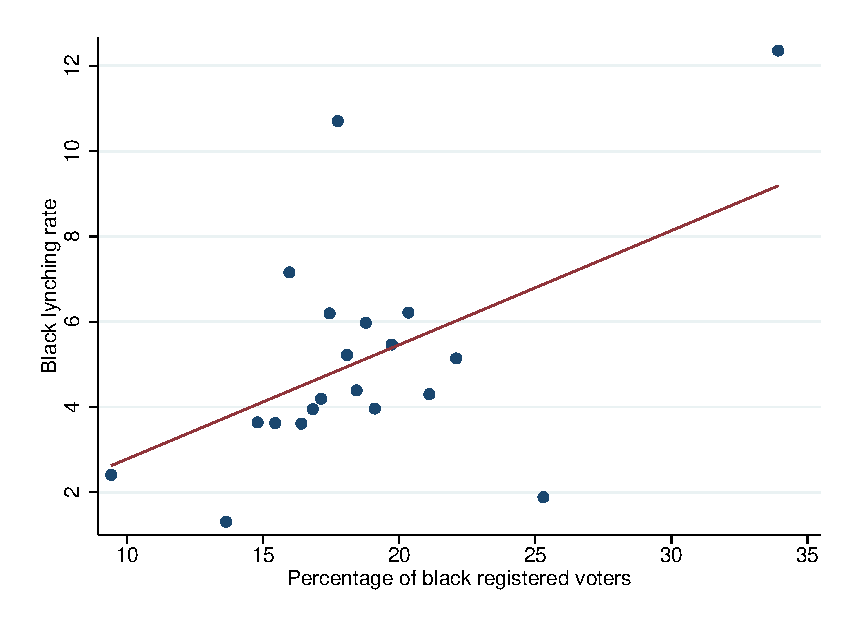
\includegraphics[height=5in,angle=0,scale=0.5]{historicalreg.eps}
			\caption{Voter Registration in 1867 and 1868 and Black Lynching Rate (County-Level)}
			\begin{figurenotes}
			Binned scatter plot. Controls for Percentage of Blacks in 1860.
			\end{figurenotes}
		\begin{figurenotes}[Source]
			Lynching data come from \citeasnoun{hal}. Voter registration data source come from John Clegg based on tables in \citeasnoun{hume2008blacks}.
		\end{figurenotes}
			\label{histreg}
\end{figure} 



\begin{figure}
		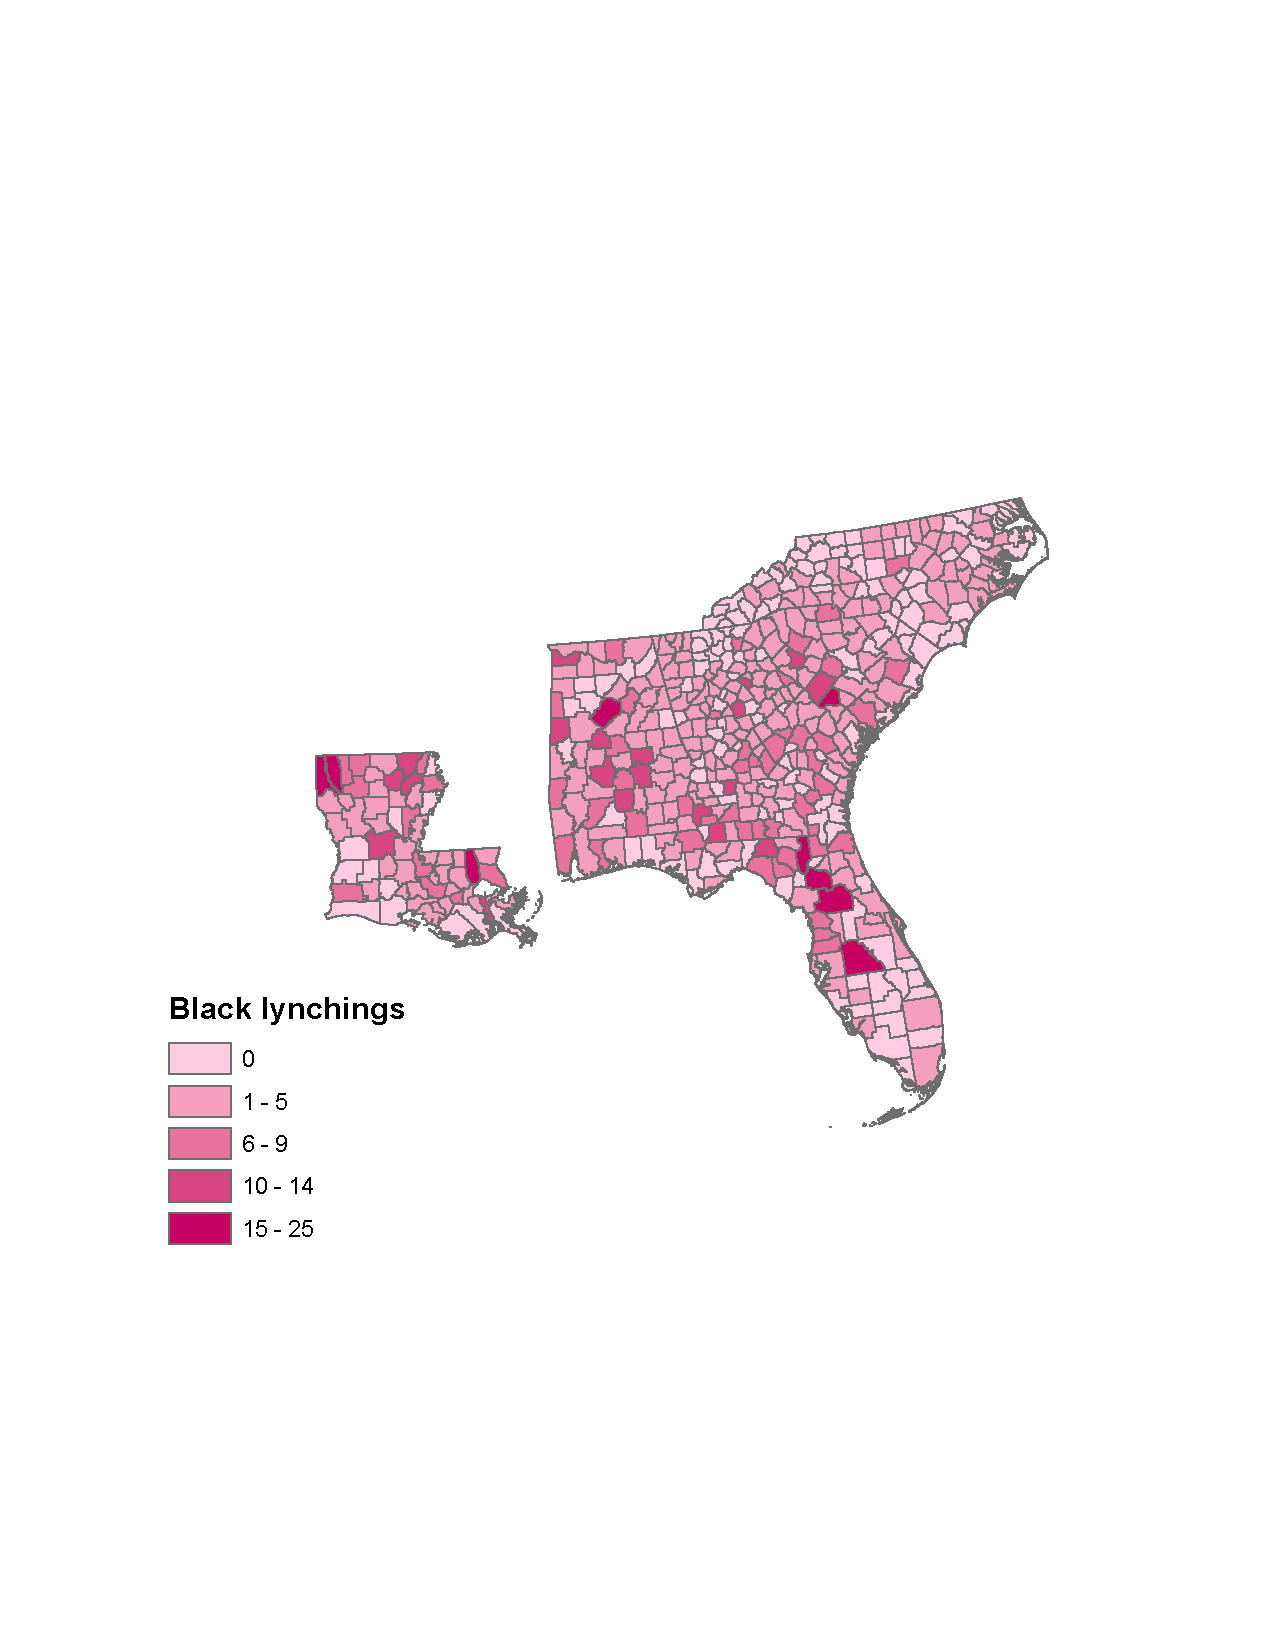
\includegraphics[height=4in,angle=0,scale=1.0]{Blacklynchmap.pdf}
		\caption{Black Lynchings}
		\begin{figurenotes}[Source]
		Lynching data come from \citeasnoun{hal}.
		\end{figurenotes}
		\label{totalmap} 
\end{figure} 
	

\begin{figure}
		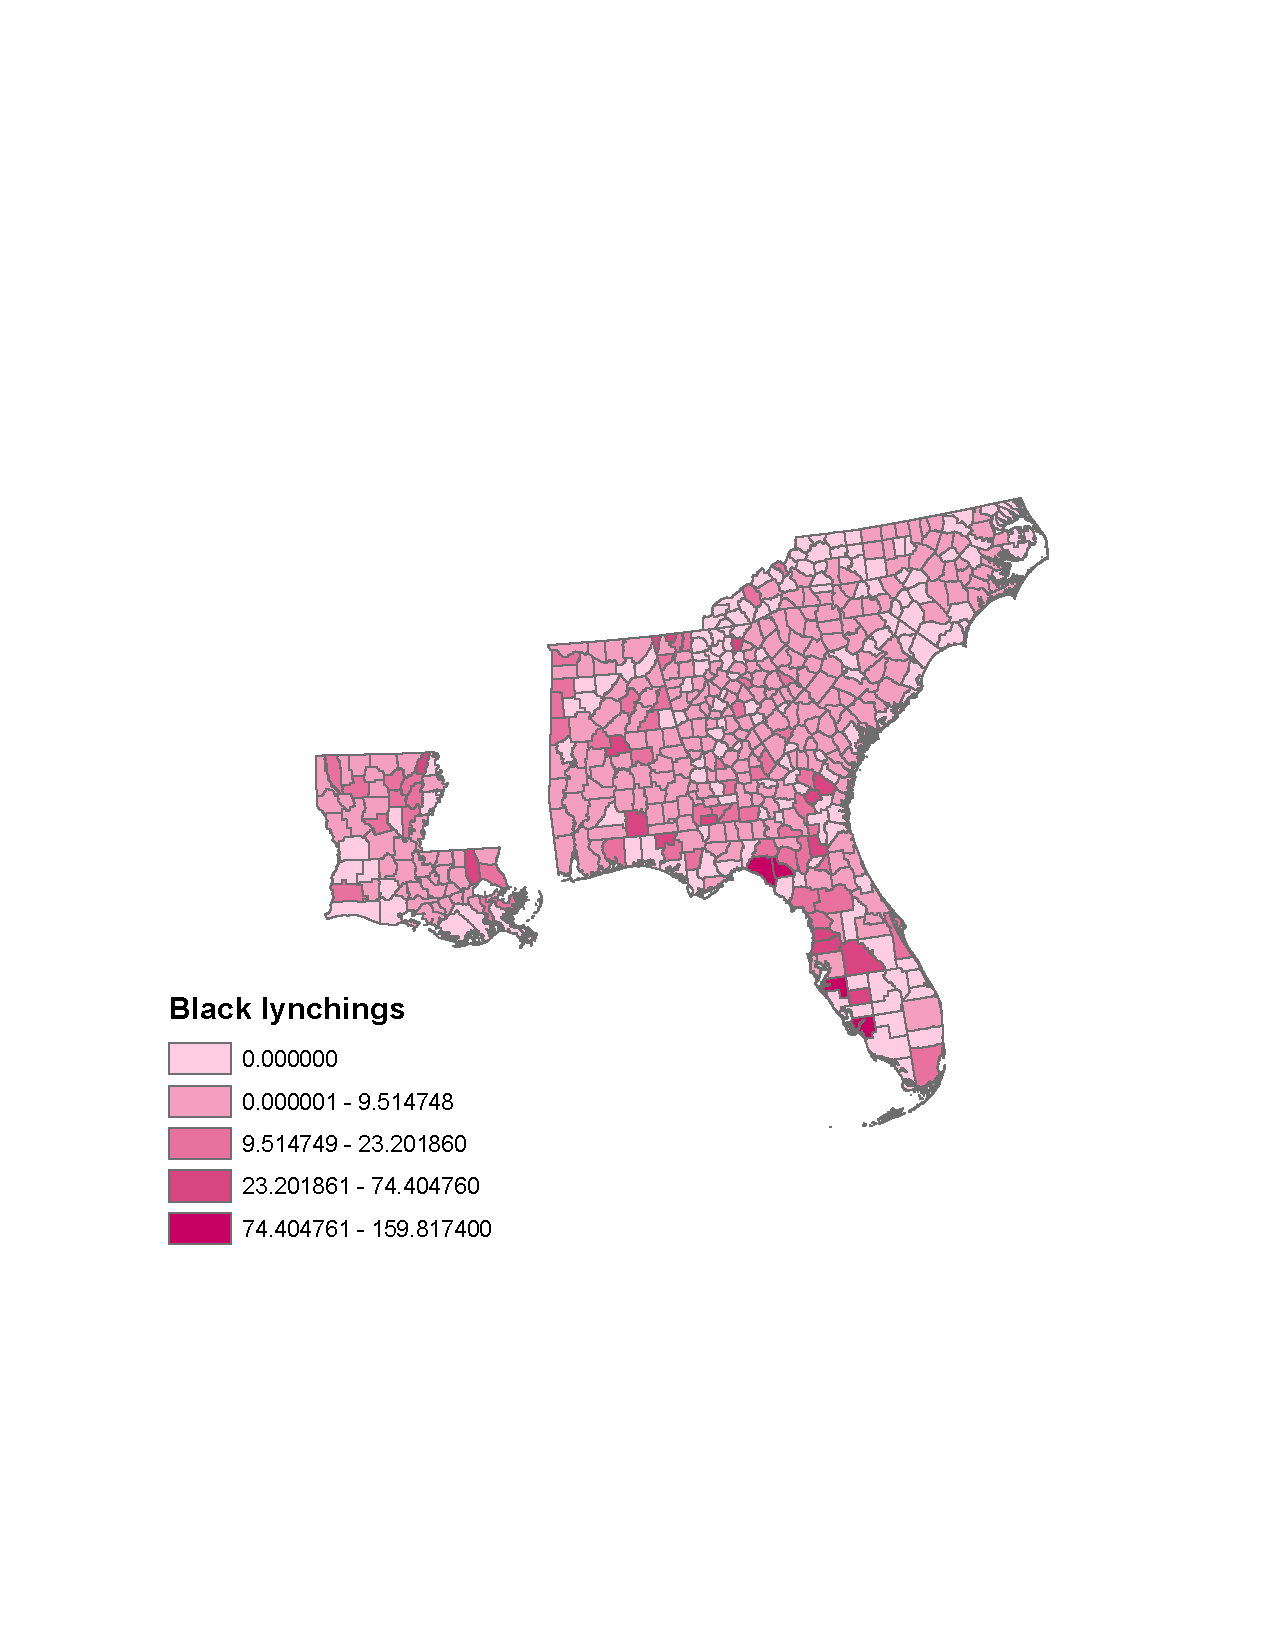
\includegraphics[height=4in,angle=0,scale=1.0]{Blacklynchpopmap.pdf}
		\caption{Black Lynchings per 10k Black Pop. in 1900}
		\begin{figurenotes}[Source]
		Lynching data come from \citeasnoun{hal}.
		\end{figurenotes}
		\label{totalnormmap} 
\end{figure} 




\begin{figure}
			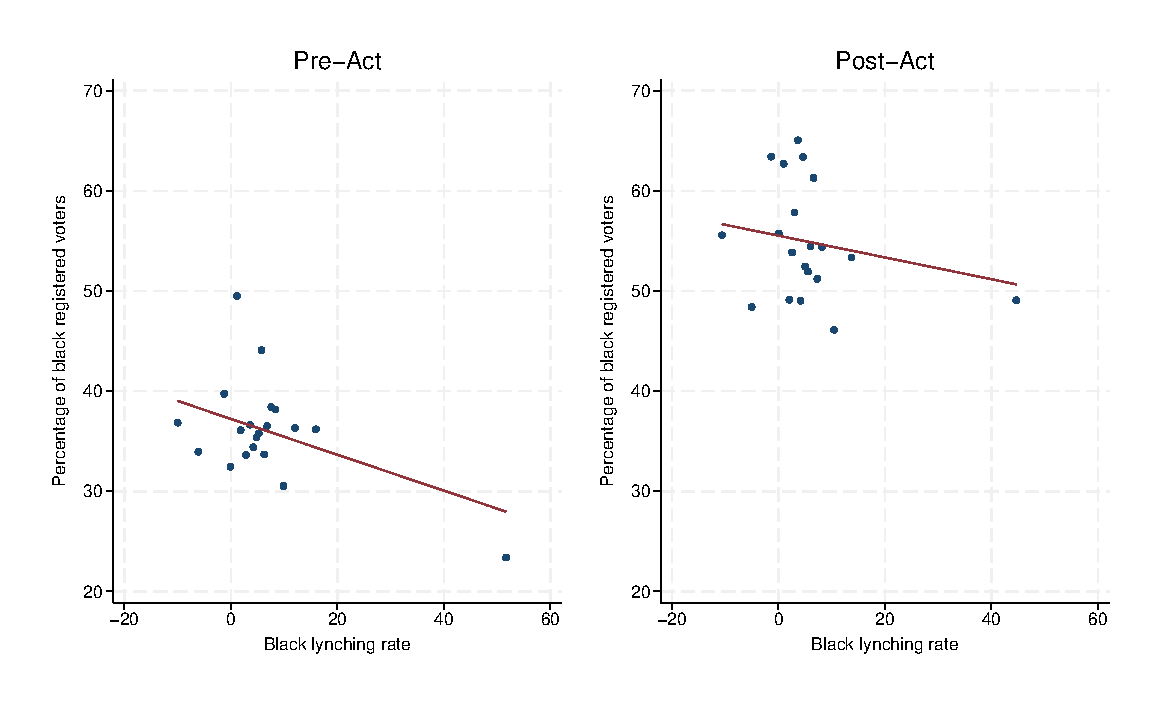
\includegraphics[height=5in,angle=0,scale=0.55]{proact.eps}
			\caption{Voter Registration Pre- and Post Voting Rights Act of 1965 and Black Lynching Rate (County-Level)}
			\begin{figurenotes}[Source]
			Lynching data come from \citeasnoun{hal}. Registration data come from \citeasnoun{proact}.
			\end{figurenotes}
			\label{proact}
\end{figure} 




\begin{figure}
			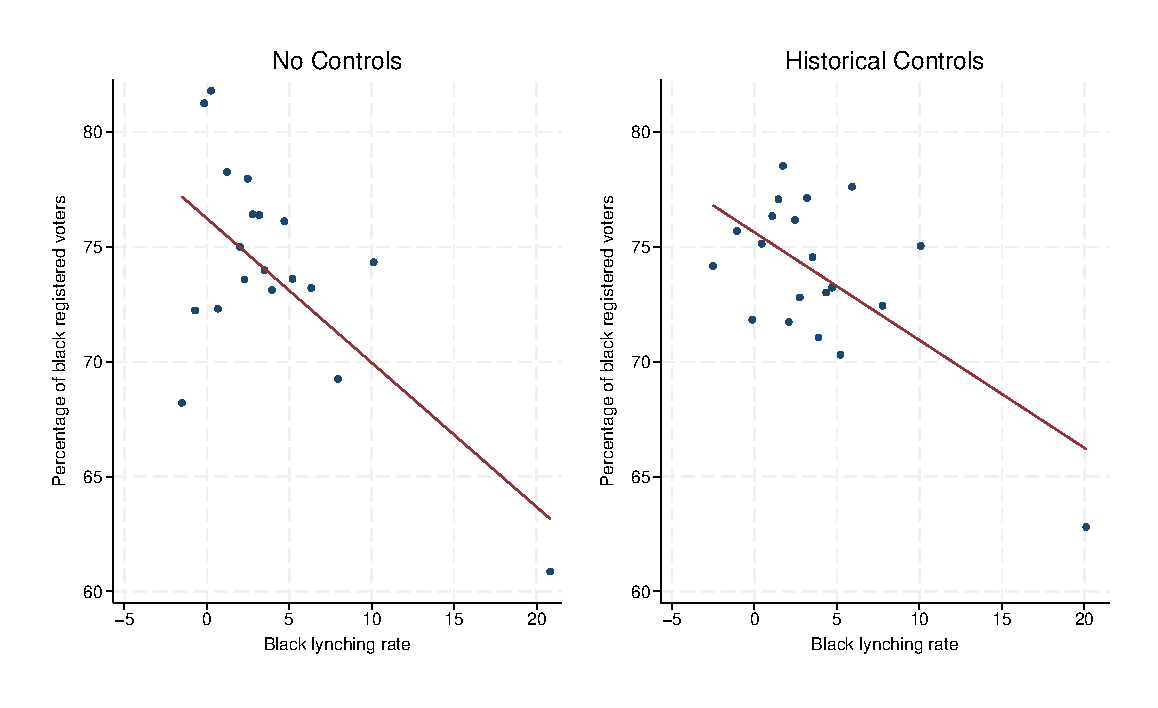
\includegraphics[height=5in,angle=0,scale=0.55]{baseline.eps}
			\caption{Lynchings and Black Voter Registration Rates}
			\begin{figurenotes}[Source]
				Lynching data come from \citeasnoun{hal}. Registered voters data come from \citeasnoun{sosal}, \citeasnoun{sosfl}, \citeasnoun{sosga}, \citeasnoun{sosla}, \citeasnoun{sosnc}, \citeasnoun{sossc}. 
			\end{figurenotes}
			\label{baseline}
\end{figure} 




\begin{figure}
		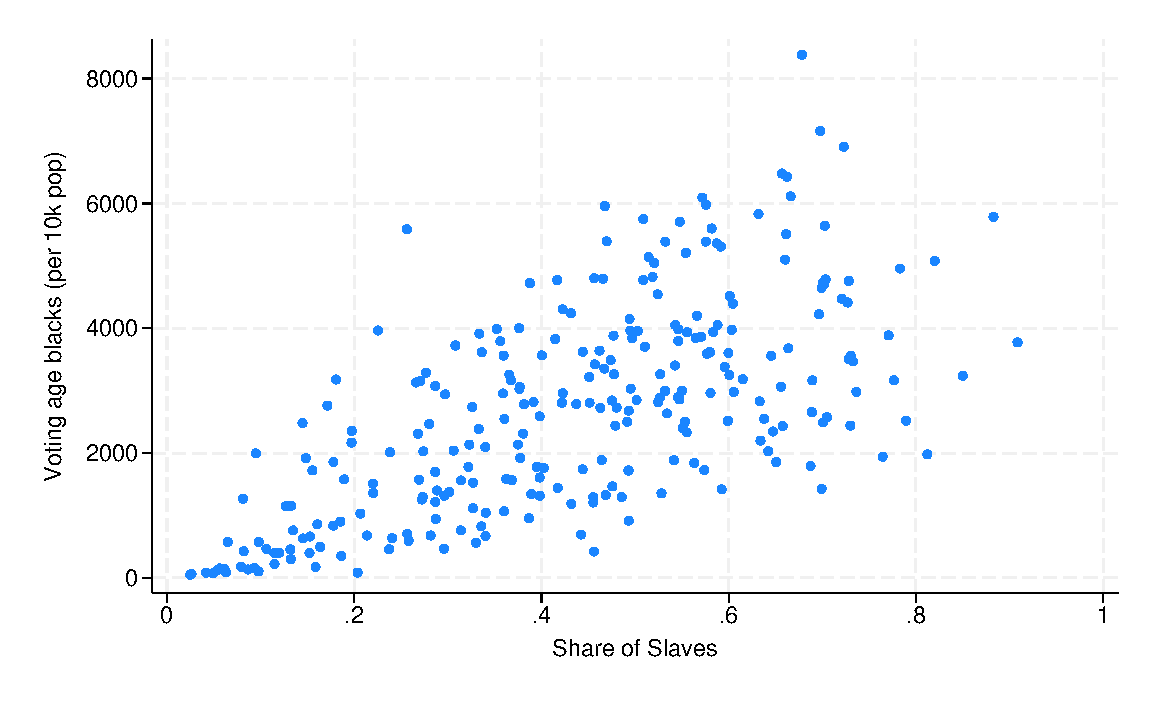
\includegraphics[height=5in,angle=0,scale=0.6]{scatblackslaves.eps}
		\caption{Scattered Plot of Contemporary Share Black and Share Slaves in 1860}
		\begin{figurenotes}[Source]
			Slave data come from \citeasnoun{ipumsnhgis}. Voting age data come from \citeasnoun{seerpop}.
		\end{figurenotes}
		\label{scatblackslaves}
\end{figure} 


\begin{figure}
		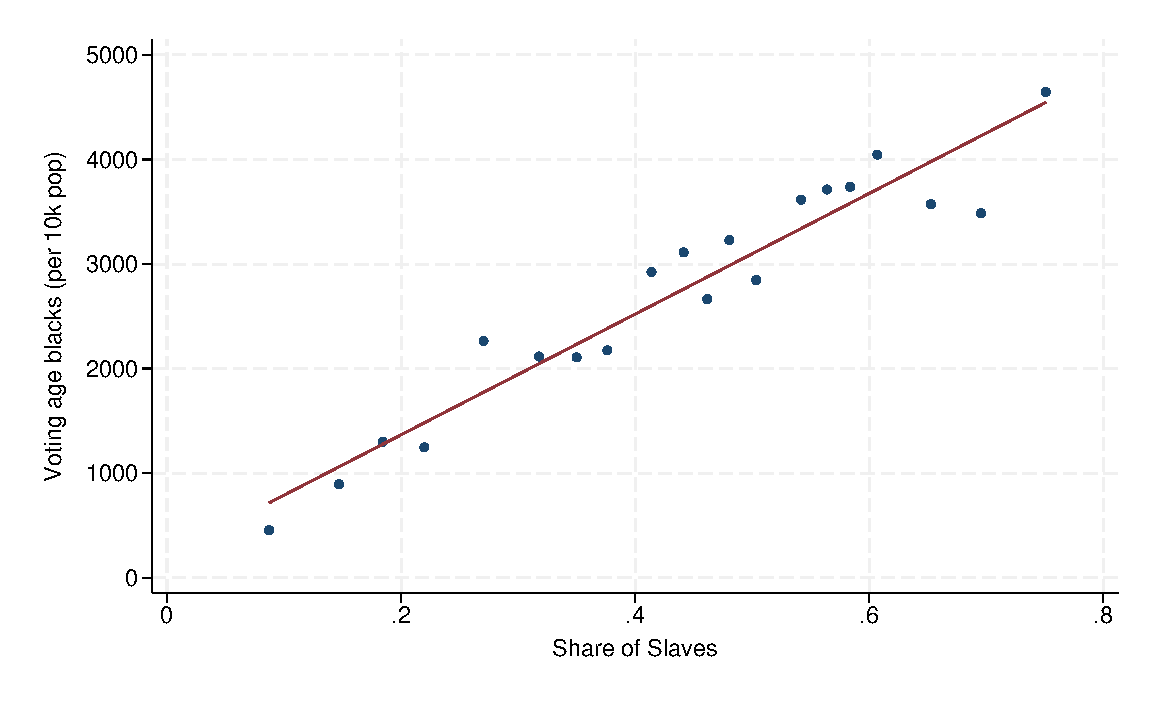
\includegraphics[height=5in,angle=0,scale=0.6]{binblackslaves.eps}
		\caption{Binned Scattered Plot of Contemporary Share Black and Share Slaves in 1860}
			\begin{figurenotes}[Source]
			Slave data come from \citeasnoun{ipumsnhgis}. Voting age data come from \citeasnoun{seerpop}.
		\end{figurenotes}
		\label{binblackslaves}
\end{figure} 

 

\begin{figure}
		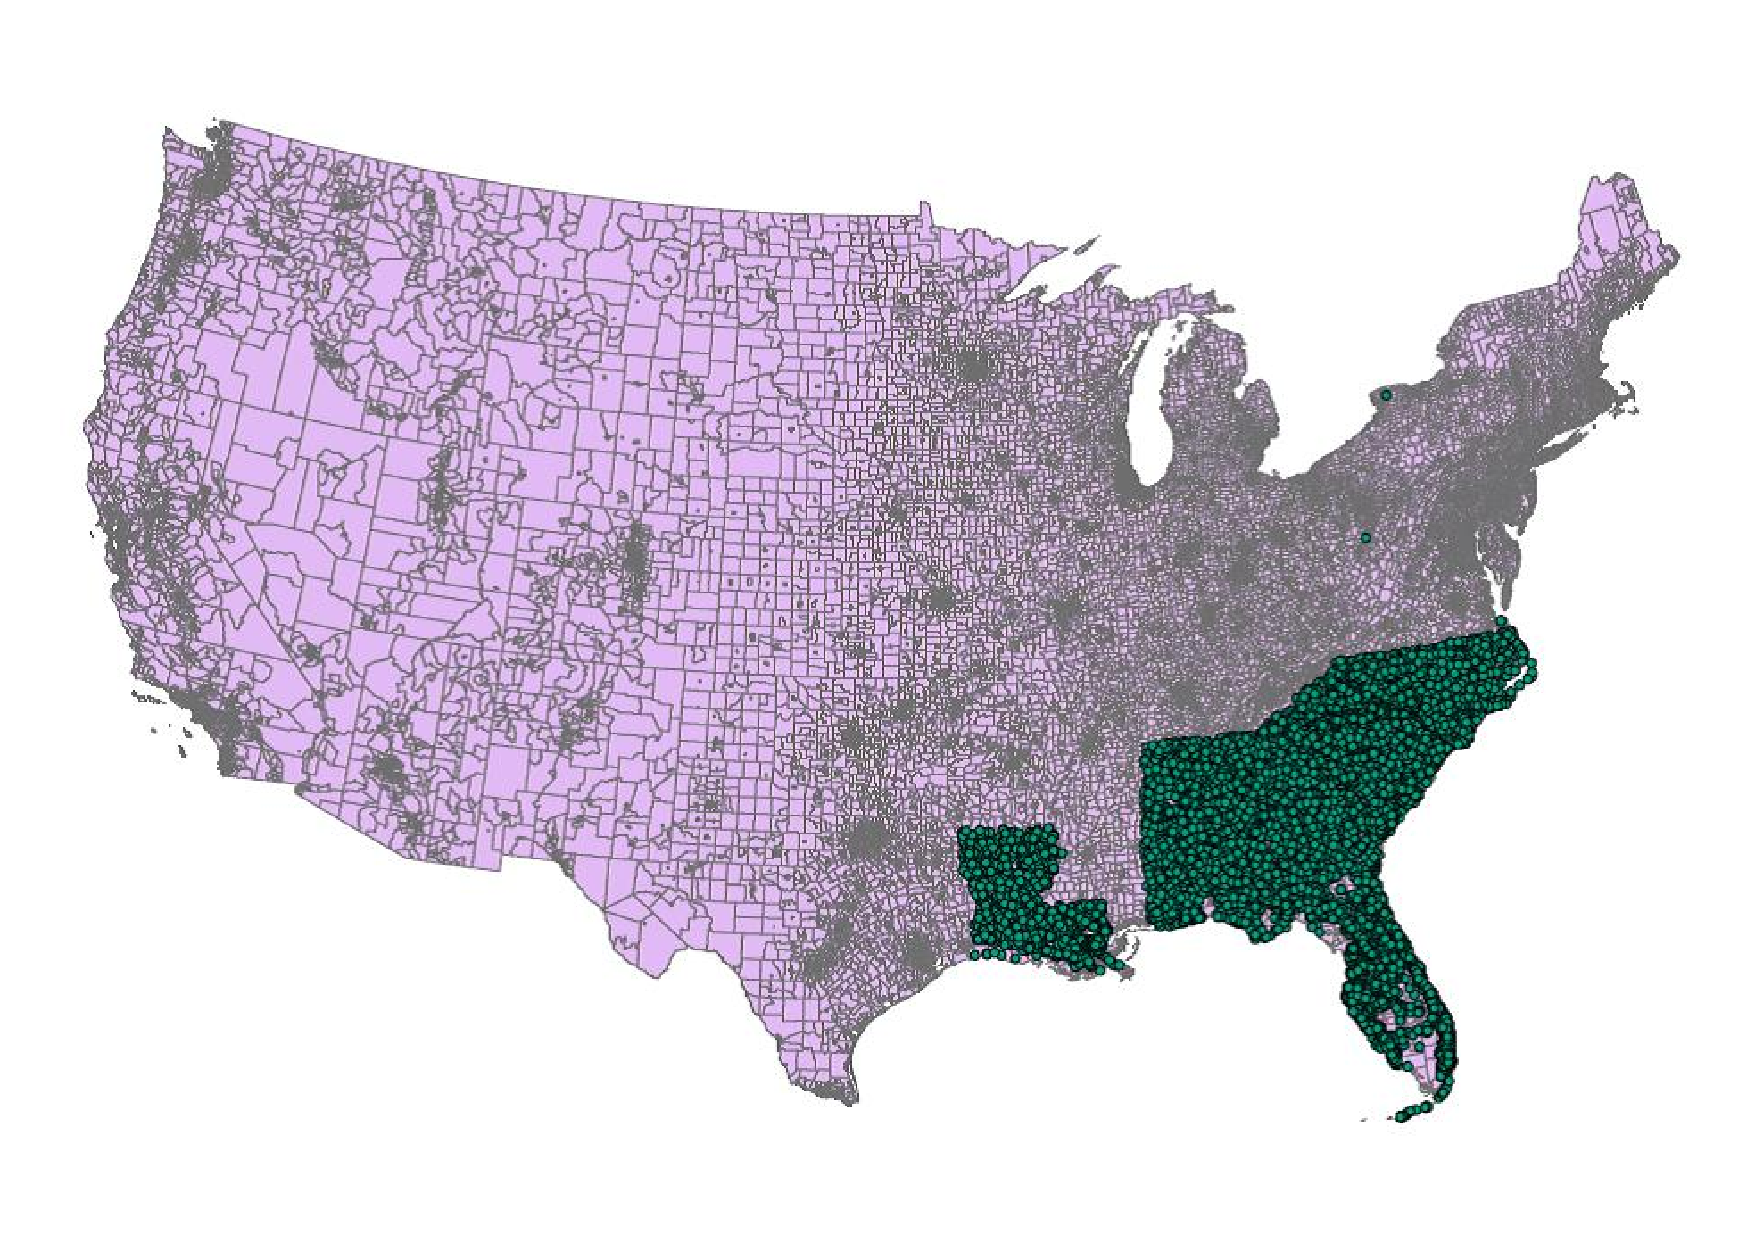
\includegraphics[height=5in,angle=0,scale=0.6]{geocodemap.pdf}
		\caption{Polling Place Locations Geocoded}
		\begin{figurenotes}[Source]
			 Polling location data come from \citeasnoun{sosalpoll}, \citeasnoun{sosflpoll}, \citeasnoun{sosgapoll}, \citeasnoun{soslapoll}, \citeasnoun{sosncpoll}, \citeasnoun{sosscpoll}. 
		\end{figurenotes}
		\label{map} 
\end{figure}


\begin{figure}
		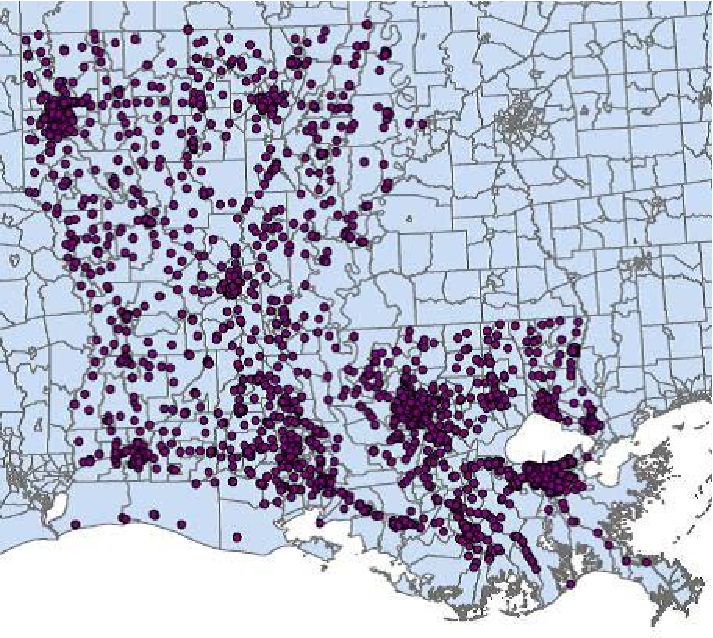
\includegraphics[height=5in,angle=0,scale=0.6]{LAMapZoom.pdf}
		\caption{Louisiana Sample Enlarged}
		\begin{figurenotes}[Source]
			Polling location data come from \citeasnoun{sosalpoll}, \citeasnoun{sosflpoll}, \citeasnoun{sosgapoll}, \citeasnoun{soslapoll}, \citeasnoun{sosncpoll}, \citeasnoun{sosscpoll}. 
		\end{figurenotes}
		\label{mapzoom} 
\end{figure}


\begin{figure}
		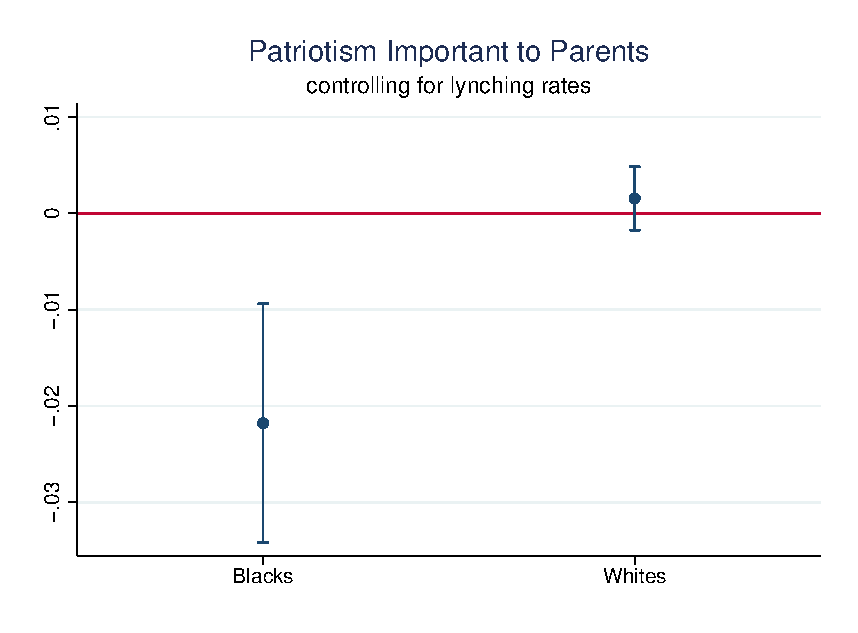
\includegraphics[height=5in,angle=0,scale=0.6]{racepat.eps}
		\caption{Cultural Voting Norms}
		\begin{figurenotes}[Source]
			Patriotism data come from \citeasnoun{sfp}.
		\end{figurenotes}
		\label{racepat}
\end{figure}


\clearpage
\bibliographystyle{aea}
\bibliography{References.lynch}



\end{document}
